\section{Morphologische Operationen}
Bei morphologischen Operationen werden die Pixel auf eine bestimmte Struktur hin untersucht.\\
Folgende Operationen sind dabei typisch:
\begin{itemize}
    \item Löschen kleiner Objekte (z.B. Pixelrauschen)
    \item Schliessen von Löchern in Objekten
    \item Zusammenfassen von räumlich nahen Objekten
    \item Löschen aller Pixel im Innern eines Objektes
    \item Reduzieren eines Objektes auf das Skelett
\end{itemize}
Für alle morphologischen Operationen ist ein Strukturelement (mit Referenz) nötig.
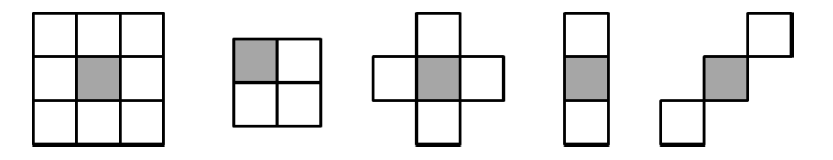
\includegraphics[width=\textwidth/3]{strukturelement.PNG}
\subsection{Erzeugen von Strukturelementen}
Matlab kennt die \lstinline{strel} Funktion um häufige Strukturelemente zu erzeugen.

\subsection{Dilatation}
Bei der Dilatation wird das Strukturelement über das Bild geschoben. Dabei werden alle Referenzpixel eingefärbt, bei welchen das Strukturelement noch ein Pixel des ursprünglichen Bilds berührt.
Das Strukturelement wird einmal an der X-Achse und einmal an der Y-Achse gespiegelt.
\begin{lstlisting}
%do a dilation 
ImageDil = imdilate(Image, StrucElem);
\end{lstlisting}

\subsection{Erosion}
Bei der Erosion werden nur diese Referenzpixel erhalten, bei welcher das Strukturelement komplett in die Struktur passt.
\begin{lstlisting}
%do an erosion 
ImageErode = imerode(Image, StrucElem);
\end{lstlisting}

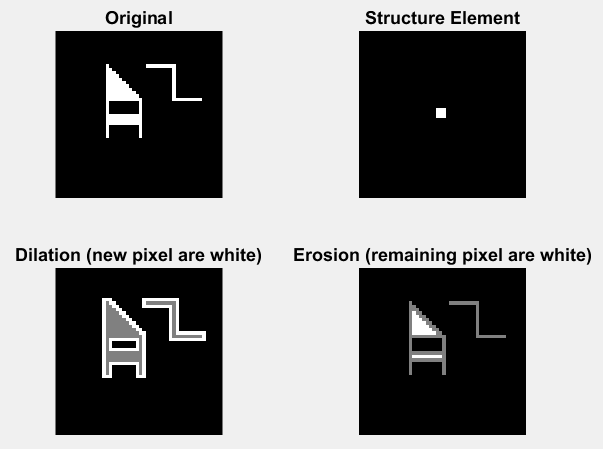
\includegraphics[width=\textwidth/3]{err_dil.PNG}

\subsection{Schliessung und Öffnung}
\begin{description}
    \item[Schliessung] Dilatation und Erosion\\
\begin{lstlisting}
ImageClose = imclose(Image, StrucElem);
\end{lstlisting}
    \item[Öffnung] Erosion und Dilatation
\begin{lstlisting}
ImageOpen = imopen(Image, StrucElem);
\end{lstlisting}
\end{description}

\subsection{Hit- und Miss-Operation}
Ein Strukturelement kann zusätzlich Bedingungen für Nachbarpixel definieren.
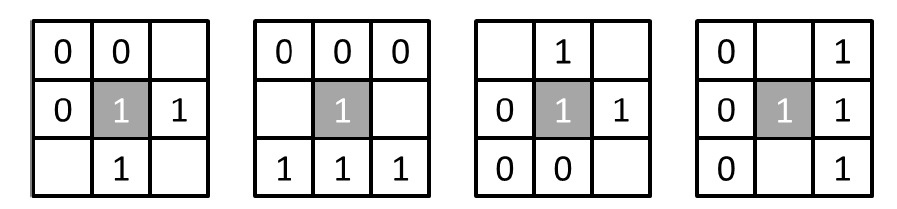
\includegraphics[width=\textwidth/3]{ext_strukturelement.PNG}
wobei:
\begin{description}
    \item[0] Das Pixel muss den Wert 0 haben
    \item[1] Das Pixel muss den Wert 255 (bzw. 1) haben
    \item['' ''] Der Wert dieses Pixels ist irrelevant (wird nicht in Betracht gezogen)
\end{description}
Durch mehrfaches Anwenden eines solchen Strukturelementes entstehen Verdünnungs- (engl. thinning) und Verdickungs-Operationen (engl. thickening).\\
Beispiel: Uebung4/Skeleton.m